\documentclass[twoside,a4paper]{report}

\usepackage{lipsum}
\usepackage[pdftex]{graphicx}
\usepackage{wrapfig}
\usepackage[font=small,labelfont=bf]{caption}
\usepackage[utf8]{inputenc}
\usepackage[polish]{babel}
\usepackage[T1]{fontenc}
\usepackage{url}
\usepackage{csquotes}
\usepackage[
sorting=none
]{biblatex}
\addbibresource{bibliografia.bib}
\usepackage{listings}
\usepackage[fit]{truncate}
\usepackage{fancyhdr}
\usepackage{multirow}
\usepackage{anysize}

\pagestyle{fancy}
\fancyhf{}

\graphicspath{ {./img/} }

\renewcommand{\lstlistlistingname}{Spis listingów}

\renewcommand{\chaptermark}[1]{\markboth{#1}{}}
\renewcommand{\sectionmark}[1]{\markright{\thesection\ #1}}
\renewcommand{\headrulewidth}{0.5pt}
\renewcommand{\footrulewidth}{0pt}

\fancyhead[LE,RO]{\bfseries\thepage}
\fancyhead[LO]{\nouppercase{\bfseries{\truncate{.95\headwidth}{\rightmark}}}}
\fancyhead[RE]{\nouppercase{\bfseries{\truncate{.95\headwidth}{\leftmark}}}}

\parskip0.05in

\marginsize{3.5cm}{2.5cm}{2.5cm}{2.5cm}
\fancyhfoffset[E,O]{0pt}

% --------------------------------------------------------------------------------

\begin{document}

% allows useg @ as a @ not as special character
% required for macro redefinition
\makeatletter

% parameters definition
% they cannot conflict with other
% like bibteh attributes etc.
\def\tytul#1{\def\@tytul{#1}}
\def\promotor#1{\def\@promotor{#1}}
\def\miasto#1{\def\@miasto{#1}}
\def\studies#1{\def\@studies{#1}}
\def\descr#1{\def\@descr{#1}}
\def\indeks#1{\def\@indeks{#1}}
\def\dept#1{\def\@dept{#1}}
\def\spec#1{\def\@spec{#1}}

\def\maketitle{
    %removal of header
    \keepXColumns
    \thispagestyle{empty}%
    \begin{center}
        \begin{tabularx}{\textwidth}{CcC}
            \multirow{4}{*}{
\includegraphics[height=2.35cm]{img/logo_pg.png}}
          & \textsc{\textbf{Politechnika Gdańska}} &
          \multirow{4}{*}{
\includegraphics[height=2.35cm]{img/logo_eti.png}}
       \\ & & \\
          & \textsc{\textbf{Wydział Elektroniki, }}& \\
          & \textsc{\textbf{Telekomunikacji i Informatyki }}& \\
        \end{tabularx}
    \end{center}
    \begin{center}
        \begin{tabularx}{\textwidth}{XX}
            \textbf{Katedra:} & \@dept\\
                              &\\
            \textbf{Imię i nazwisko dyplomanta:} & \@author\\
                                                 &\\
            \textbf{Nr albumu:} & \@indeks\\
                                &\\
            \textbf{Forma i poziom studiów:} & \@studies\\
                                             &\\
            \textbf{Kierunek studiów:} & Informatyka\\
                                       &\\
            \textbf{Specjalność:} & \@spec
        \end{tabularx}
    \end{center}
    \begin{center}
        \Large{\textbf{Praca dyplomowa magisterska}}
    \end{center}
    \vspace{1cm}
    \begin{tabular}{l}
        \textbf{Temat pracy:} \\ \@tytul\\
        \\
        \textbf{Title of thesis:} \\ \@title\\
        \\
        \textbf{Opiekun pracy:} \\ \@promotor\\
        \\
        \textbf{Data ostatecznego zatwierdzenia raportu podobieństw w JSA:} TBA
    \end{tabular}
    \vspace*{\stretch{6}}
    \begin{center}
        \@miasto, \@date
    \end{center}

}

%restore @ sign
\makeatother

\cleardoublepage


\title{Wykorzystanie języka ELM do tworzenia aplikacji frontendowych.}
\author{Marcin Jurczak}
\date{2022}
\miasto{Gdańsk}
\promotor{dr\ inż.\ Krzysztof Manuszewski}
\studies{Stacjonarne jednolite studia magisterskie}
\indeks{171641}
\dept{Algorytmów i Technologii Internetowych}

\maketitle

% --------------------------------------------------------------------------------

\chapter*{Streszczenie}
\lipsum[1]

\textbf{Słowa kluczowe:} Elm, programowanie funkcyjne, wytwarzane aplikacji internetowych

\textbf{Dziedzina nauki i techniki: }Nauki inżynieryjne i techniczne, inżynieria informatyczna.

{\let\clearpage\relax\chapter*{Abstract}}
\lipsum[1]

\textbf{Keywords:} Elm, functional programming, web development

\textbf{Field of Science and Technology:} Engineering and Technology, Information engineering.

% spis treści
\tableofcontents

% --------------------------------------------------------------------------------

\chapter{Wstęp i cel pracy}

Celem niniejszej pracy jest zapoznanie się z funkcyjnym językiem programowania Elm, porównanie go z powszechnymi rozwiązaniami do tworzenia aplikacji frontendowych, a także przygotowanie instrukcji laboratoryjnej, która mogłaby zostać potencjalnie wykorzystana w ramach przedmiotu Współczesne Aplikacje Programowania Funkcyjnego, prowadzonego przez mojego promotora, dra inż. Krzysztofa Manuszewskiego.

W drugim rozdziale chciałbym się skupić na przedstawieniu

% --------------------------------------------------------------------------------

\chapter{Aplikacje frontendowe}

\section{Powszechne rozwiązania}

\subsection{React}
\cite{react}
\cite{reactdocs}
\subsection{Angular}
\cite{angularjs}
\cite{angulardocs}
\subsection{Vue.js}
\cite{vuejsdocs}


% --------------------------------------------------------------------------------

\chapter{Programowanie funkcyjne}

% --------------------------------------------------------------------------------

\chapter{Elm}
Elm~\cite{elmdocs} jest czysto funkcyjnym językiem programowania przeznaczonym do tworzenia graficznych interfejsów użytkownika. Powstał w roku 2012 wraz z opublikowaniem przez Evana Czaplickiego pracy ,,Elm: Concurrent FRP for Functional GUIs''~\cite{Czaplicki2012ElmC}. Podczas jego tworzenia nacisk został położony na użyteczność, wydajność oraz niską podatność na błędy.

\section{The Elm Architecture}
\textit{The Elm Architecture} jest schematem tworzenia interaktywnych aplikacji internetowych lub gier.
\begin{figure}[h]
    \centering
    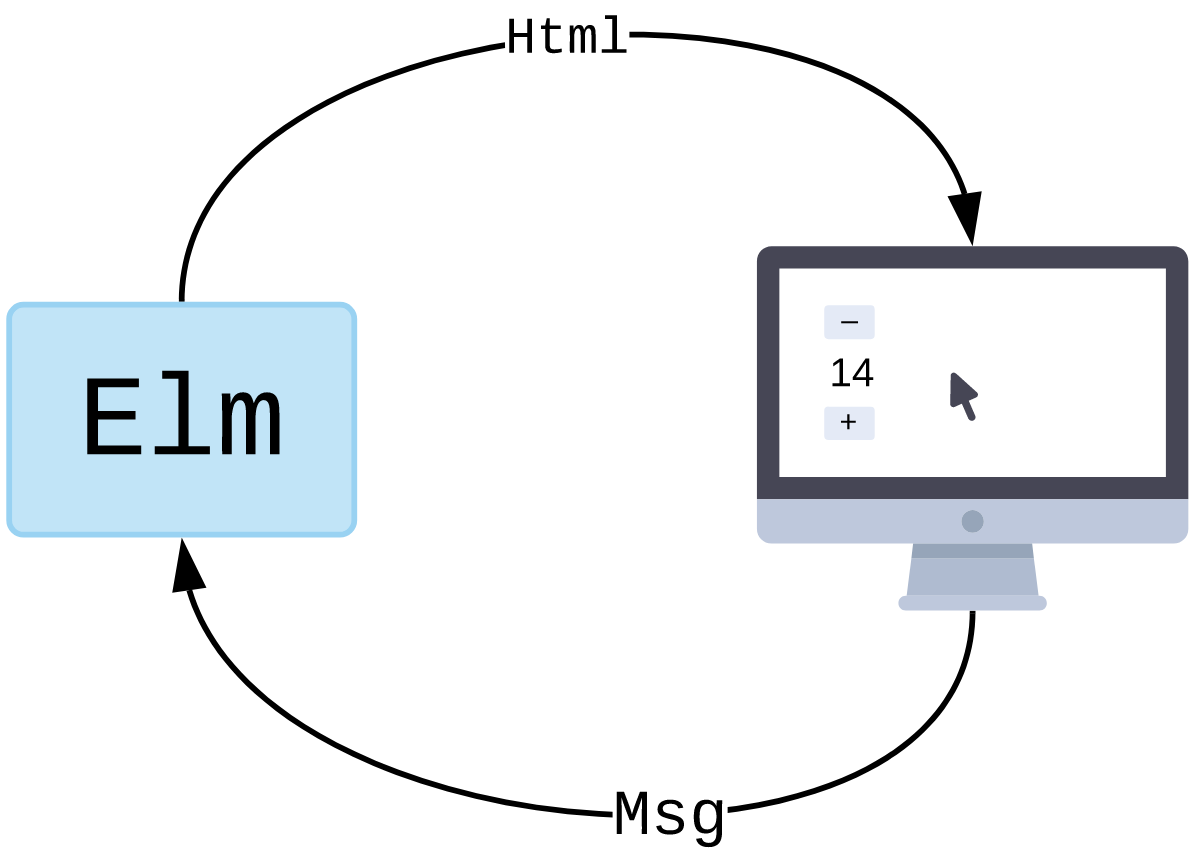
\includegraphics[width=0.6\textwidth]{elm_arch.png}
    \caption{The Elm Architecture}
    \label{fig:elm_arch}
\end{figure}

Architektura Elma składa się z trzech podstawowych elementów:
\begin{itemize}
    \setlength\itemsep{-0.1em}
    \item Model -- opisujący stan aplikacji
    \item Update -- opisujący logikę aplikacji
    \item View -- opisujący wygląd aplikacji
\end{itemize}

\subsection{Model}
\begin{minipage}{.45\textwidth}
Celem modelu jest zdefiniowanie danych w naszej aplikacji. W tym przypadku model będzie bardzo prosty - jedna wartość liczbowa, która może zostać zwiększona lub zmniejszona.
\end{minipage}\hfill
\begin{minipage}{.45\textwidth}
\lstset{frame=single}
\begin{lstlisting}[caption={\textit{The Elm Architecture} - Model},label=kod:Model]
type alias Model = Int


init : Model
init =
  0
\end{lstlisting}
\end{minipage}\hfill

\subsection{Update}
\begin{minipage}{.45\textwidth}
\lstset{frame=single}
\begin{lstlisting}[caption={\textit{The Elm Architecture} - Update},label=kod:Update]
type Msg
  = Increment
  | Decrement


update : Msg -> Model -> Model
update msg model =
  case msg of
    Increment ->
      model + 1

    Decrement ->
      model - 1
\end{lstlisting}
\end{minipage}\hfill
\begin{minipage}{.45\textwidth}
Funkcja update ma za zadanie opisywać jak nasz model będzie się zmieniał w czasie. Może odebrać dwa typy wiadomości - Increment i Decrement. W wyniku operacji update otrzymujemy nowy, zaktualizowany model.
\end{minipage}\hfill
\subsection{View}
Funkcja view jako argument przyjmuje model i zwraca kod HTML. Wykorzystany został tutaj handler onClick, który po kliknięciu generuje odpowiednią wiadomość. Znak plusa generuje wiadomość Increment, znak minusa Decrement. Wybrana wiadomość trafia do funkcji update.

\lstset{frame=single}
\begin{lstlisting}[caption={\textit{The Elm Architecture} - View},label=kod:View]
view : Model -> Html Msg
view model =
  div []
    [ button [ onClick Decrement ] [ text "-" ]
    , div [] [ text (String.fromInt model) ]
    , button [ onClick Increment ] [ text "+" ]
    ]
\end{lstlisting}

\section{Narzędzia}

\paragraph{elm repl}

\paragraph{elm init}

\paragraph{elm reactor}

\paragraph{elm make}

\paragraph{elm install}


% --------------------------------------------------------------------------------

\chapter{Instrukcja laboratoryjna}
W poniższym rozdziale przedstawiam przykładową instrukcję laboratoryjną, która krok po kroku przeprowadza czytelnika przez proces tworzenia aplikacji w Elmie, zaczynając od przygotowania środowiska deweloperskiego, przez podstawy języka wraz z ćwiczeniami pozwalającymi na lepsze zrozumienie składni, aż po stworzenie większej aplikacji frontendowej.

\section{Instalacja środowiska}

\subsection{Linux}

\subsection{Windows}

\section{Podstawy języka Elm}

\section{Aplikacja frontendowa}

% --------------------------------------------------------------------------------

\chapter{Podsumowanie}
\section{Wnioski}

% --------------------------------------------------------------------------------

\listoffigures
% \listoftables
\lstlistoflistings

\printbibliography
% \bibliographystyle{plain}
% \bibliography{bibliografia}

% --------------------------------------------------------------------------------

\end{document}
